% vim: ai sw=2 spell spelllang=cs

\documentclass[xcolor=dvipsnames,handout]{beamer}

\let\Oldemph\emph
\renewcommand{\emph}[1]{\textcolor{blue}{\Oldemph{#1}}}
\newcommand{\heading}[1]{\textbf{\textcolor{BurntOrange}{#1}}}
\newcommand{\header}[1]{\textbf{\texttt{\textcolor{WildStrawberry}{#1}}}}
\newcommand{\doc}[1]{\textbf{\texttt{\textcolor{OliveGreen}{#1}}}}

\mode<presentation>
{
\usetheme{Madrid}
}

\setbeamertemplate{navigation symbols}{}

\uselanguage{czech}
\deftranslation[to=czech]{Section}{Sekce}
\deftranslation[to=czech]{Subsection}{Podsekce}

\usepackage[czech]{babel}
\usepackage[utf8x]{inputenc}
\usepackage{helvet}
\usepackage{mathptmx}
\usepackage[IL2]{fontenc}
\usepackage{graphicx}
\usepackage{hyperref}
\usepackage[final]{listings}
\usepackage{multirow}
\usepackage{tikz}
\usepackage{pgfplots} 
\usepackage[absolute,overlay]{textpos}
\usepackage{xspace}
\usetikzlibrary{arrows, positioning}

\tikzset{tl_state/.style={rounded corners, thick, draw, minimum height=6mm,
	minimum width=12mm, bottom color=black!15, top color=black!5}}
\tikzset{tl_phase/.style={thick, draw, minimum size=8mm}}
\tikzset{tl_edge/.style={<-, >=stealth', semithick}}

\lstset{tabsize=2,numbers=none,showstringspaces=false,breaklines=true,
	breakatwhitespace=true,escapeinside={(*@}{@*)},
	basicstyle=\scriptsize,keywordstyle=\bfseries\color{OliveGreen},
	commentstyle=\color{blue}, columns=flexible, language=C}

\newcommand{\cmd}[2][]{\lstinline[columns=fullflexible, language=bash,
	basicstyle=\ttfamily, #1]$#2$}
\newcommand{\code}[2][]{\lstinline[columns=fullflexible, basicstyle=\ttfamily,
	#1]$#2$}
\newcommand{\file}[2][]{\code[language=XML, #1]{#2}}

\newcommand{\xes}{\texttt{x86}\xspace}

\title{Linuxové jádro}
\subtitle{Včera, dnes a zítra}
\date{4. 12. 2013}

\author{Jiri Slaby}

\institute[ITI, FI]{ITI, Fakulta informatiky}

\begin{document}

\begin{frame}
  \titlepage
\end{frame}

\section{Úvod}

\begin{frame}
  \frametitle{Úvodní informace}

  \heading{Přednášející}
  \begin{itemize}
    \item Student Fakulty informatiky (Bc., Mgr.\ a PhD.)
    \item Vývojář jádra od r.\ 2005 (NetBSD, Linux)
  \end{itemize}

  \pause
  \bigskip

  \heading{Prezentace}
  \begin{itemize}
    \item Úvod do jádra
    \item Volná diskuze
  \end{itemize}

\end{frame}

\begin{frame}
  \frametitle{Přehled prezentace}

  \tableofcontents
\end{frame}

\begin{frame}
  \frametitle{Co to je Linuxové jádro?}

  \begin{itemize}
    \item Monolitické jádro
    \begin{itemize}
      \item S podporou modulů
      \item Dvouúrovňové zabezpečení
    \end{itemize}

    \pause

    \item Zdrojové kódy v GNU C a assembleru

    \item Licence: GPLv2 (kromě firmware)

    \pause

    \item Kde jádro najdu?
    \begin{itemize}
      \item Hlavní stránka: \url{http://www.kernel.org/}
      \item Aktuální strom: \url{http://git.kernel.org/}
      \item \emph{A u svých distributorů}
    \end{itemize}
  \end{itemize}

\end{frame}

\section{Historie}
\frame{\sectionpage}

\subsection{První zmínky}

\begin{frame}[fragile]
  \frametitle{První zmínky}

  \heading{Linus Torvalds v roce 1991 na \texttt{comp.os.minix}:}
\begin{verbatim}
I'm doing a (free) operating system
(just a hobby, won't be big and
professional like gnu) for 386(486)
AT clones.
\end{verbatim}

\pause

\begin{verbatim}
... It is NOT portable ...
\end{verbatim}

\pause

\begin{verbatim}
... and it probably never will support
anything other than AT-harddisks ...
\end{verbatim}

\end{frame}

\subsection{Vývoj za 20 let}

\begin{frame}
  \frametitle{Milníky 0.01--1.2}

  \begin{itemize}
    \item Verze: 0.01 (1991)
    \begin{itemize}
      \item První vydaná verze
      \item Pouze limitovaná podpora HW
      \item (stále ke stažení)
    \end{itemize}

    \pause

    \item Verze: 0.11 (1991)
    \begin{itemize}
      \item Lze na něm zkompilovat jádro
    \end{itemize}

    \pause

    \item Verze: 0.95 (1992)
    \begin{itemize}
      \item Podpora X
    \end{itemize}

    \pause

    \item Verze 1.0 (1994)
    \begin{itemize}
      \item ,,Komponenty jsou plně vyspělé''
      \item RedHat a SUSE vydávají distribuce 1.0
    \end{itemize}

    \pause

    \item Verze 1.2 (1995)
    \begin{itemize}
      \item Podpora modulů
    \end{itemize}

  \end{itemize}

\end{frame}

\begin{frame}
  \frametitle{Milníky 2.0--3.0}

  \begin{itemize}
    \item Verze 2.0 (1996)
    \begin{itemize}
      \item SMP a podpora více procesorů
    \end{itemize}

    \pause

    \item Verze 2.2 (1999)
    \begin{itemize}
      \item Podpora multimédií (v4l)
    \end{itemize}

    \pause

    \item Verze 2.4 (2001)
    \begin{itemize}
      \item Podpora USB, PCMCIA a další
    \end{itemize}

    \pause

    \item Verze 2.6 (2003)
    \begin{itemize}
      \item Nový plánovač O(1)
      \begin{itemize}
	\item Umí být preemptivní
	\item Nativní vlákna NPTL
      \end{itemize}
      \item Zvukový podsystém ALSA
    \end{itemize}

    \pause

    \item Verze 3.0 (2011)
    \begin{itemize}
      \item 20.\ výročí jádra 
      \item Žádné převratné změny
      \item Spíše kratší jméno pro 2.6.40
    \end{itemize}

  \end{itemize}

\end{frame}

\begin{frame}
  \frametitle{Hlavní větev}

  \begin{itemize}
    \item Stabilní 2.x řady: 2.0, 2.2, 2.4, 2.6
    \item Nestabilní 2.x řady: 2.1, 2.3, 2.5
    \begin{itemize}
      \item Sloužily k začleňování vlastností
    \end{itemize}

    \pause

    \item 2--3 \emph{roky} $\Rightarrow$ příliš dlouhá doba
    \begin{itemize}
      \item Kód vývojářů se nepoužívá
      \item Uživatelé nemají nové vlastnosti
      \item Distributoři musejí používat kód z nestabilní větve
    \end{itemize}

    \pause

    \item Už žádná nestabilní řada (2.7)
    \begin{itemize}
      \item Vše do 2.6
      \item Každé 2--3 \emph{měsíce} nové jádro

      \pause

      \item A příliš se nevzdálit od stability
    \end{itemize}

    \pause

    \item Verzování
    \begin{itemize}
      \item 2.x: a.b.c
      \item 3.0: a.b
    \end{itemize}
  \end{itemize}

\end{frame}

\begin{frame}
  \frametitle{Stabilní stromy}

  \begin{itemize}
    \item Nutnost opravovat chyby ve vydaných 2.6.x
    \begin{itemize}
      \item Distribuce mívají fixní verzi jádra
    \end{itemize}

    \pause

    \item Záplata se pošle s ,,Cc: stable''
    \item Ale: první do aktuálního 2.6.y, potom do 2.6.x

    \pause

    \item Verzování
    \begin{itemize}
      \item 2.6: a.b.c.d
      \item 3.0: a.b.c
    \end{itemize}
  \end{itemize}

\end{frame}

\section{Současnost}
\frame{\sectionpage}

\begin{frame}[fragile]
  \frametitle{Správa kódu}

  \begin{verbatim}
The problem is that Linus doesn't scale.
\end{verbatim}

  \bigskip
  \pause

  \heading{Nástroje pro správu}
  \begin{itemize}
    \item V minulosti
    \begin{itemize}
      \item \textsc{Diff} (do 2.4)
      \item \textsc{BitKeeper} (do 2.6.12)
      \item \textsc{Mercurial} (průběžně)
    \end{itemize}

    \pause

    \item Dnes
    \begin{itemize}
      \item Převážně \textsc{Git}
      \item Jen s historií do 2.6.12
    \end{itemize}

    \pause

    \item Celá historie jádra v \textsc{Gitu} existuje
    \begin{itemize}
      \item \nolinkurl{full-history-linux}
    \end{itemize}
  \end{itemize}

\end{frame}

\subsection{Vývojový model}

\begin{frame}[fragile]
  \frametitle{Vývojový model}

  \heading{Nahoře je jeden Torvalds, který začleňuje sady záplat}
\begin{verbatim}
There aren't enough swear-words in
the English language, so now I'll
have to call you perkeleen vittupää
just to express my disgust and
frustration with this crap.
\end{verbatim}

  \pause
  \bigskip

  \heading{Správci podsystémů sbírají záplaty a posílají žádost nahoru}

\end{frame}

\begin{frame}[fragile]
  \frametitle{Stabilní rozhraní}

  \heading{Stabilní ABI}
  \begin{itemize}
    \item Staré jádro \emph{by mělo} běžet na nových systémech
    \item A opačně

    \pause

    \item Pravidlo číslo jedna: nerozbíjíme uživatelské rozhraní
  \end{itemize}

\begin{verbatim}
Shut up, Mxxxx. And I don't _ever_
want to hear that kind of obvious
garbage and idiocy from a kernel
maintainer again. Seriously.
...
WE DO NOT BREAK USERSPACE!
\end{verbatim}

\end{frame}

\begin{frame}[fragile]
  \frametitle{Nestabilní rozhraní}

  \heading{Nestabilní API}
  \begin{itemize}
    \item Linuxové jádro je vyvíjeno rychle
    \item Často se přepisuje kód
    \item \code{device_create} se měnilo od 2.6.0 5$\times$ 
    \item Kód je jednoduše použitelný
  \end{itemize}

\begin{verbatim}
You think you want a stable kernel
interface, but you really do not,
and you don't even know it.
\end{verbatim}

\end{frame}

\begin{frame}
  \frametitle{Používané nástroje}

  \heading{Překlad}
  \begin{itemize}
    \item \textsc{Gcc}
    \begin{itemize}
      \item Alespoň verze 3.2
      \item Včetně LTO
    \end{itemize}

    \pause

    \item \textsc{IntelCC}
    \begin{itemize}
      \item Úspešnost kolísá
    \end{itemize}

    \item \textsc{Clang}
    \begin{itemize}
      \item Stále neúplná podpora
    \end{itemize}
  \end{itemize}

  \pause
  \medskip

  \heading{Ostatní}
  \begin{itemize}
    \item GNU \textsc{Make}, \textsc{Binutils}, \textsc{Perl}, \dots
  \end{itemize}

\end{frame}

\begin{frame}[fragile]
  \frametitle{Hello World}

  \begin{center}
  \begin{tabular}{c|c}
  \file{Makefile} & \file{hello.c} \\
  \begin{lstlisting}[language=make]
KDIR=/lib/modules/$(shell uname -r)/build
KBUILD=$(MAKE) -C $(KDIR) M=$(PWD)

obj-m := hello.o

default:
        $(KBUILD) modules

clean:
        $(KBUILD) clean
  \end{lstlisting} &

  \pause

  \begin{lstlisting}
#include <linux/module.h>

static int my_init(void)
{
       	printk(KERN_INFO "Hello World\n");
        return 0;
}

static void my_exit(void)
{
}

module_init(my_init);
module_exit(my_exit);
  \end{lstlisting}
  \end{tabular}

  \bigskip
  \bigskip
  \pause

  \heading{Více v PB173}
  \end{center}
\end{frame}

\begin{frame}
  \frametitle{Hotplug a jádro}

  \begin{itemize}
    \item Většina sběrnic podporuje hotplug
    \begin{itemize}
      \item PCI, USB, PC Card, CPU
    \end{itemize}
    \item Ne všechny ovladače

    \item Některé subsystémy nepodporují hotremove
    \begin{itemize}
      \item Paměť
    \end{itemize}
  \end{itemize}

\end{frame}


\subsection{Podporované platformy}

\begin{frame}
  \frametitle{Podporované platformy}

  \begin{itemize}
    \item Hlavní architektury
    \begin{itemize}
      \item ARM, IA-64, PowerPC, s390, x86
    \end{itemize}

    \pause

    \item Ostatní
    \begin{itemize}
      \item Alpha, Blackfin, AVR32, m68k, MIPS, Microblaze, Sparc a další
    \end{itemize}

    \pause

    \item Údajně běží na
    \begin{itemize}
      \item 95 \% TOP500 superpočítačů (2013)
      \item 42 \% všech počítačových/mobilních zařízení (2012)
    \end{itemize}
  \end{itemize}

  \pause
  \bigskip

  ,,Běží téměř na všem, z čeho trčí nožičky''

\end{frame}

\subsection{Statistiky}
\frame{\subsectionpage}

\begin{frame}
  \frametitle{Počet řádků kódu}

  \begin{center}
  \begin{tikzpicture}
  \begin{axis}[
    width=\textwidth,
    height=0.8\textheight,
    xtick={1,2,3,4,5,6,7,8},
    xticklabels={0.01,1.0,2.0,2.2,2.4,2.6,3.0,3.12},
    ticklabel style={/pgf/number format/fixed}
  ]
  \addplot coordinates {
    (1, 10239)   % 0.01
    (2, 176250)  % 1.0
    (3, 400000)  % 2.0 guess
    (4, 1800847) % 2.2
    (5, 3377902) % 2.4
    (6, 5929913) % 2.6
    (7, 14647033) % 3.0
    (8, 16727762) % 3.12
  };
  \end{axis}
  \end{tikzpicture}
  \end{center}

  3.12: 16'727'762 řádků kódu

\end{frame}

\begin{frame}
  \frametitle{Změny za den}

  \begin{center}
  \begin{tikzpicture}
  \begin{axis}[
    width=\textwidth,
    height=0.8\textheight,
    xtick={1,2,3,4,5,6,7,8,9,10,11,12,13,14},
    xticklabels={13,16,19,22,25,28,31,34,37,0,3,6,9,12},
    ticklabel style={/pgf/number format/fixed}
  ]
  \addplot coordinates {
    ( 1, 53.48)  % 6.13
    ( 2, 69.73)  % 6.16
    ( 3, 92.85)  % 6.19
    ( 4, 87.01)  % 6.22
    ( 5, 147.51) % 6.25
    ( 6, 119.05) % 6.28
    ( 7, 118.29) % 6.31
    ( 8, 116.58) % 6.34
    ( 9, 150.61) % 6.37
    (10, 143.02) % 3.0
    (11, 142.57) % 3.3
    (12, 144.32) % 3.6
    (13, 172.61) % 3.9
    (14, 176.24) % 3.12
  };
  \end{axis}
  \end{tikzpicture}
  \end{center}

  3.12: změněno 7,3 řádků za \emph{hodinu}

\end{frame}

\begin{frame}
  \frametitle{Počet přispěvatelů}

  \begin{center}
  \begin{tikzpicture}
  \begin{axis}[
    width=\textwidth,
    height=0.8\textheight,
    xtick={1,2,3,4,5,6,7,8,9,10,11,12,13,14},
    xticklabels={13,16,19,22,25,28,31,34,37,0,3,6,9,12},
    ticklabel style={/pgf/number format/fixed}
  ]
  \addplot coordinates {
    ( 1, 545)  % 6.13
    ( 2, 709)  % 6.16
    ( 3, 801)  % 6.19
    ( 4, 870)  % 6.22
    ( 5, 1123) % 6.25
    ( 6, 1075) % 6.28
    ( 7, 1166) % 6.31
    ( 8, 1150) % 6.34
    ( 9, 1273) % 6.37
    (10, 1133) % 3.0
    (11, 1246) % 3.3
    (12, 1223) % 3.6
    (13, 1389) % 3.9
    (14, 1333) % 3.12
  };
  \end{axis}
  \end{tikzpicture}
  \end{center}

  3.12: 1333 přispěvatelů

\end{frame}

\begin{frame}
  \frametitle{Z pohledu firem}

  \begin{itemize}
    \item Přispívající z asi 200 firem
    \item Počet je takřka neměnný od 2.6.25 (2008)

    \pause

    \item Rozdělení
    \begin{itemize}
      \item Neznámo (47 \%)
      \item RedHat (11 \%)
      \item Novell (9 \%)
      \item Linux Foundation (8 \%)
      \item IBM, Intel, Oracle, \dots
    \end{itemize}
  \end{itemize}

\end{frame}

\begin{frame}
  \frametitle{Rok jaderného vývojáře}

  \begin{center}
    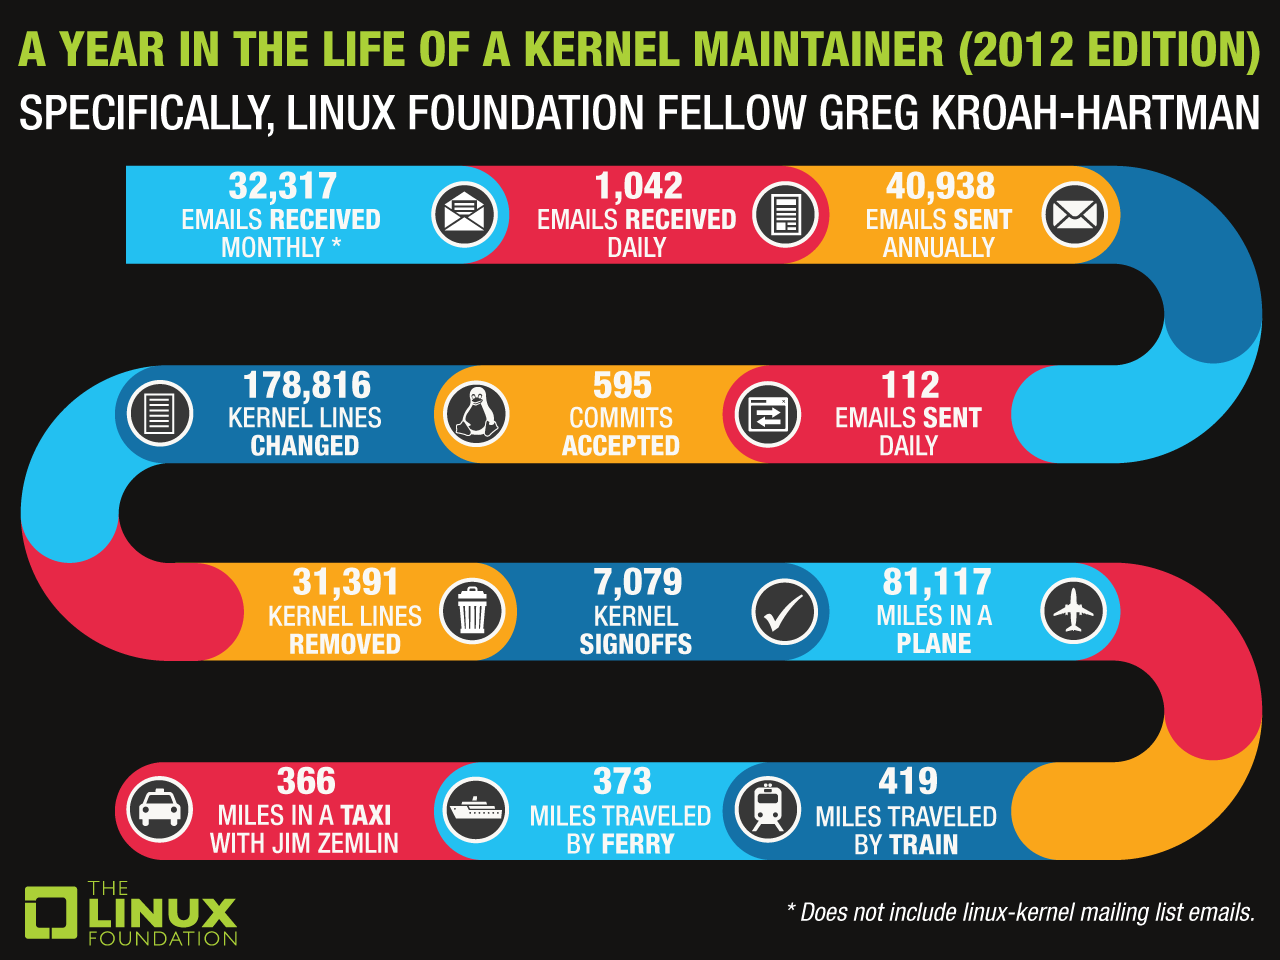
\includegraphics[height=0.85\textheight]{gregkh2012}
  \end{center}

\end{frame}

\subsection{Testy kvality}

\begin{frame}
  \frametitle{Testy kvality}

  \begin{itemize}
    \item Velmi omezeně samotnými vývojáři
    \begin{itemize}
      \item Často jen překlad
      \item Nástroje typu \textsc{Sparse}
    \end{itemize}

    \pause

    \item Automatická analýza
    \begin{itemize}
      \item Intel robot (\texttt{kbuild test robot <fengguang.wu@intel.com>})
      \begin{itemize}
	\item \texttt{warning: zpráva z překladače}
      \end{itemize}

      \pause

      \item \textsc{Coverity Prevent}
      \begin{itemize}
	\item \texttt{New Defects reported by Coverity Scan for Linux}
      \end{itemize}

      \pause

      \item Projekt Linux driver verifier
      \begin{itemize}
	\item Snaží se opravovat sami
	\item \texttt{Found by Linux Driver Verification project}
      \end{itemize}

      \pause

      \item Různé statické analyzátory
      \begin{itemize}
	\item \textsc{Smatch}, \textsc{Stanse}, \dots
      \end{itemize}
    \end{itemize}

    \pause

    \item Řádné Q\&A až u distributorů
      \begin{itemize}
	\item Mnohdy až enterprise
      \end{itemize}
  \end{itemize}

\end{frame}

\section{Budoucnost}
\frame{\sectionpage}

\begin{frame}
  \frametitle{Záplatování za běhu}
  
  \heading{Chceme 24/7, ale bezpečně}
  \begin{itemize}
    \item Oracle a \textsc{Ksplice}
    \begin{itemize}
      \item Všechny CVE záplaty
      \item Podpora jen Oracle Enterprise
      \item Pro RHEL jen trial
      \item Na githubu je funkční klon
    \end{itemize}

    \pause

    \item Intel (Andi Kleen)
    \begin{itemize}
      \item Záplatování uživatelského prostoru
      \item \code{ptrace}
    \end{itemize}

    \pause

    \item Pravděpodobně nezůstane jen u toho
    \begin{itemize}
      \item Parallels?
    \end{itemize}
  \end{itemize}
\end{frame}

\begin{frame}
  \frametitle{Virtualizace}

  \begin{itemize}
    \item \textsc{cgroups}
    \begin{itemize}
      \item \textsc{systemd} je ,,znásilnilo''
      \item Je třeba přepsat (Tejun Heo)
    \end{itemize}

    \pause

    \item \textsc{XEN}
    \begin{itemize}
      \item Dlouholetý záměr začlenit \textsc{XEN}
      \item Jádro už může běžet jako dom0
    \end{itemize}
  \end{itemize}

\end{frame}

\begin{frame}
  \frametitle{Co bude v 3.13?}

  \heading{Z těch hlavních}
  \begin{itemize}
    \item Procesory
    \begin{itemize}
      \item Podpora pro 64bitový ARM
      \item x86 a podpora 8192 procesorů
    \end{itemize}

    \pause

    \item \textsc{nftables}
    \begin{itemize}
      \item \textsc{iptables}, \textsc{ip6tables}, \textsc{arptables} a
	\textsc{ebtables} dohromady
      \item Budou dostupné současně
      \item Kompatibilní vrstva pro existující pravidla
    \end{itemize}

    \pause

    \item Vícenásobná I/O fronta
    \begin{itemize}
      \item Lepší podpora SSD disků
      \item Nezávislé I/O fronty rozprostřené přes více CPU
    \end{itemize}
  \end{itemize}

\end{frame}

\section{Závěr}

\begin{frame}
  \frametitle{Závěr}

  \begin{center}
    \Large
    \heading{Jádro je docela živý ekosystém}
  \end{center}

\end{frame}

\subsection{Diskuze}

\begin{frame}
  \frametitle{Konec prezentace}

  \huge
  \begin{center}
  Děkuji za pozornost \\[1em]
  Volná diskuze\dots
  \end{center}

\end{frame}

\end{document}

